Na rys.~\ref{fig:2} przedstawiono wyniki
eksperymentu~\ref{subsec:rhodobacter}.
W 10 dniu eksperymentu widoczny jest istotny
statystycznie spadek \acrshort{od}\textsubscript{600}
w próbkach o $c_{\acrshort{ww}} = 80$ \% względem próbek
o niższych stężeniach.
Oznacza to hamowanie wzrostu \textit{R. sphaeroides}
przy stężeniach \acrshort{ww} 80 \%.
Z~tego względu w kolejnych eksperymentach kultywowano
\textit{R. sphaeroides} na \acrshort{m27} + 50 \% \acrshort{ww}\@.
Rys.~\ref{fig:3} przedstawia wyniki
eksperymentu~\ref{subsec:mlra}.
Dla BG-11 oraz \acrshort{ww}2 zaobserwowano początkową wysoką
aktywność \acrshort{mlra} i jej późniejszy spadek, natomiast
w przypadku \acrshort{ww}3 początkowa aktywność była bliska 0,
a następnie wzrosła w czasie hodowli.
Na rys.~\ref{fig:4} przedstawiono wyniki pomiarów
napięcia w eksperymencie~\ref{subsec:volt}.
Z wykresu wynika, że największe napięcia generowane
są w przypadku hodowli \textit{R. sphaeroides}
o \acrshort{od}\textsubscript{600} w zakresie od 0.200 do 0.535,
przy czym hodowle gęstsze, o~\acrshort{od}\textsubscript{600} bliskim
0.500 wykazują spadki napięcia po dłuższym czasie.

\begin{figure}[t!]
    \centering
    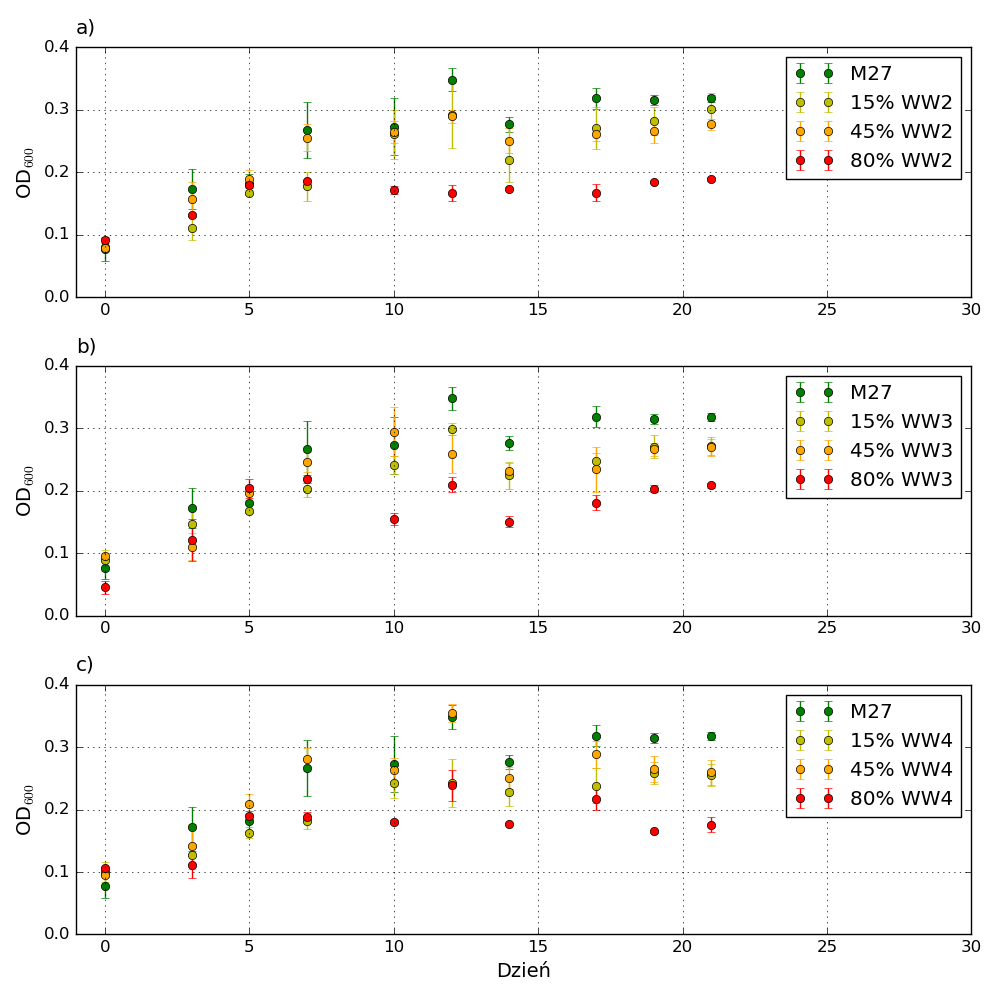
\includegraphics[width=13cm]{figures/ww}
    \caption{
        Zmiany \acrshort{od}\textsubscript{600} hodowli \textit{R. sphaeroides} w czasie w \acrshort{m27}:
        \textbf{a}~zawierającym \acrshort{ww}2 w~stężeniach 15 \%, 45 \% i 80 \%;
        \textbf{b}~zawierającym \acrshort{ww}3 w stężeniach 15 \%, 45 \% i 80 \%;
        \textbf{c}~zawierającym \acrshort{ww}4 w stężeniach 15 \%, 45 \% i 80 \%.
        Słupki błędów to \acrshort{sem} (n = 3).
    }
    \label{fig:2}
\end{figure}

\vspace{\fill}

\begin{figure}[b!]
    \centering
    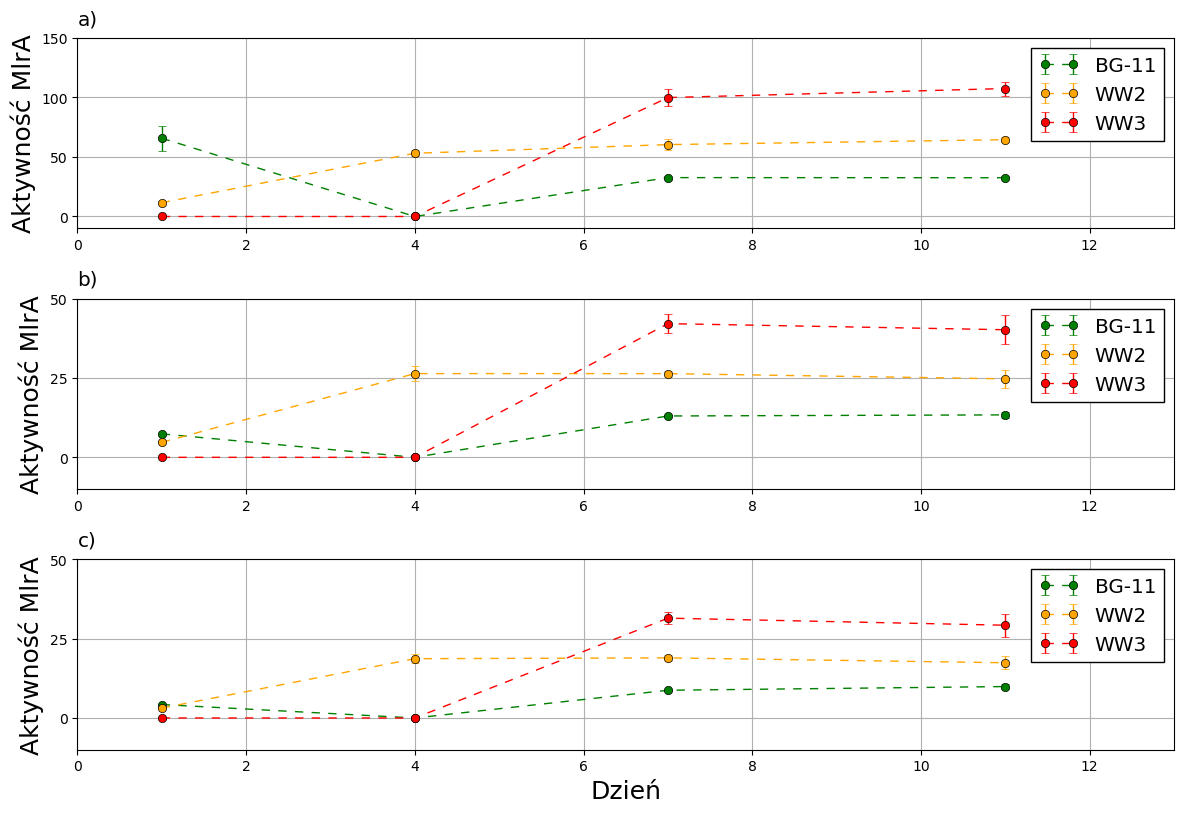
\includegraphics[width=13cm]{figures/mlra_activity}
    \caption{
        Aktywność \acrshort{mlra} w lizatach komórek
        \textit{Synechocystis sp.} PCC 6803 McCormick 7
        kultywowanych z użyciem różnych rodzajów \acrshort{ww} zmieszanych
        w proporcjach 1:1 z BG-11 jako pożywki. Słupki błędów to \acrshort{sem} (n = 3).
        Aktywność przeliczono na całkowitą zawartość białka w lizatach.
        Pomiar białka przeprowadzono w próbkach rozcieńczonych
        a) 20x; b) 50x; c) 100x. DO ZMIANY!!!!!

    }
    \label{fig:3}
\end{figure}

\begin{figure}[h!]
    \centering
    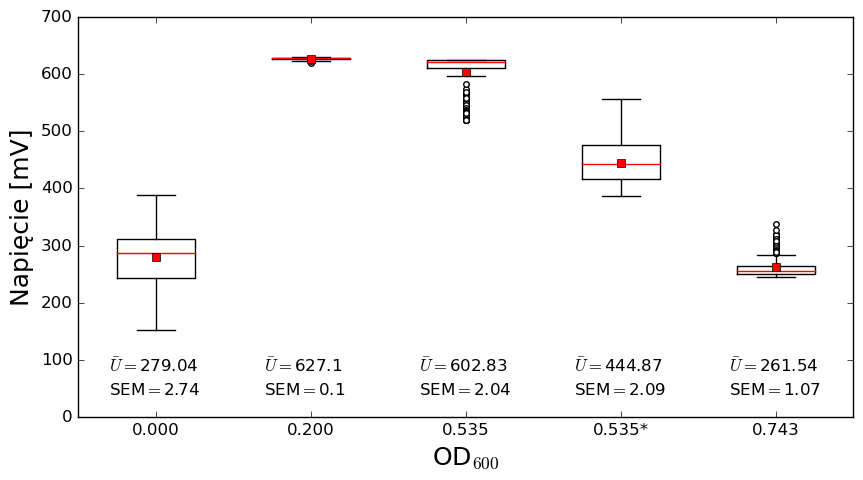
\includegraphics[width=12cm]{figures/mfc-volt-boxplt}
    \caption{
        Wykres pudełkowy przedstawiający wyniki pomiaru napięcia prądu stałego ($U$)
        w czasie w zależności od \acrshort{od}\textsubscript{600} hodowli
        \textit{R. sphaeroides} znajdującej się w komorze z anodą.
        Uwzględnione zostały wartości ze 160 punktów pomiarowych rejestrowanych co 1 min.
        Czerwonym kwadratem oznaczono wartość średniej arytmetycznej napięcia
        ($\bar{U}$) dla danej serii.
        Czerwoną linią oznaczona została wartość mediany danej serii pomiarowej.
        Punkty odbiegające zostały oznaczone czarnymi kółeczkami.
        * oznacza pomiar wykonany po 24 h adaptacji komórek \textit{R. sphaeroides} do elektrody.
    }
    \label{fig:4}
\end{figure}
